    \chapter{Introduction to Hardware and Software components}
    This chapter serves as an introduction to the frameworks, software, and libraries we use. The work we present can be simplified explained as a knowledge base containing parameters that a robot can use to perform specific actions.

    Firstly, we would like to introduce the robotic component, which acts as the interface between the knowledge base we have created and the robot, followed by an introduction to ontologies and knowledgebases.
    \section{Robotic section: ROS and PyCRAM}
    
    The main framework we use is \textit{PyCRAM} \cite{pycram}, which serves as an interface for various software components such as knowledge, perception, or manipulation. 
	This framework utilizes another framework, \textit{ROS} (Robotic Operating System) \cite{ros}, to communicate with the different robot components. These two frameworks are now introduced in the following.    
    \subsection{ROS}
	\label{sec:ROS}
    \begin{wrapfigure}{r}{0.5\textwidth}
        \centering
        
\includegraphics[width=0.48\textwidth]{Graphics/ROS.jpg}
		\caption{ROS \cite{ros}}
    \end{wrapfigure}

    \textit{ROS} \cite{ros}, which stands for Robot Operating System, is an open-source middleware framework designed to develop and control robots. Despite its name, \textit{ROS} \cite{ros} is not a traditional operating system but rather a set of software libraries and tools that help in building and managing robot software. It provides a standardized and modular approach to developing robotic systems, allowing for easier collaboration and code reuse in the robotics community.
    Key features and components of \textit{ROS} \cite{ros} include:
    \begin{itemize}
        \item \textbf{Nodes}: \textit{ROS} \cite{ros} systems are organized into nodes, which are individual processes that perform specific tasks. Nodes communicate with each other by passing messages over topics, creating a decentralized and modular architecture.
        \item \textbf{Topics}: Nodes exchange data through topics, which are named buses over which messages are passed. This publish/subscribe communication model allows for asynchronous and loosely coupled interactions between nodes.
        \item \textbf{Launch files}: \textit{ROS} \cite{ros} uses launch files to specify how to start multiple nodes and configure the system. This helps simplify the setup of complex robotic systems.
        \item \textbf{Master}: The ROS Master is responsible for managing the communication between nodes by keeping track of publishers, subscribers, and services. It facilitates the discovery and connection of nodes within a \textit{ROS} \cite{ros} network.
    \end{itemize}

    \subsection{Pr2}
	\label{sec:pr2}
	Introduced in 2010 by Willow Garage, the \textit{PR2} \cite{pr2} stands as an advanced research robot. Boasting multiple joints and 20 degrees of freedom, this robot excels in autonomous navigation and the manipulation of a diverse array of objects, making it an ideal choice for our specific needs. Additionally, it is equipped with a \textit{HeadStereoCamera} that can be used to perceive the surroundings.
	
    \begin{figure}[H]
    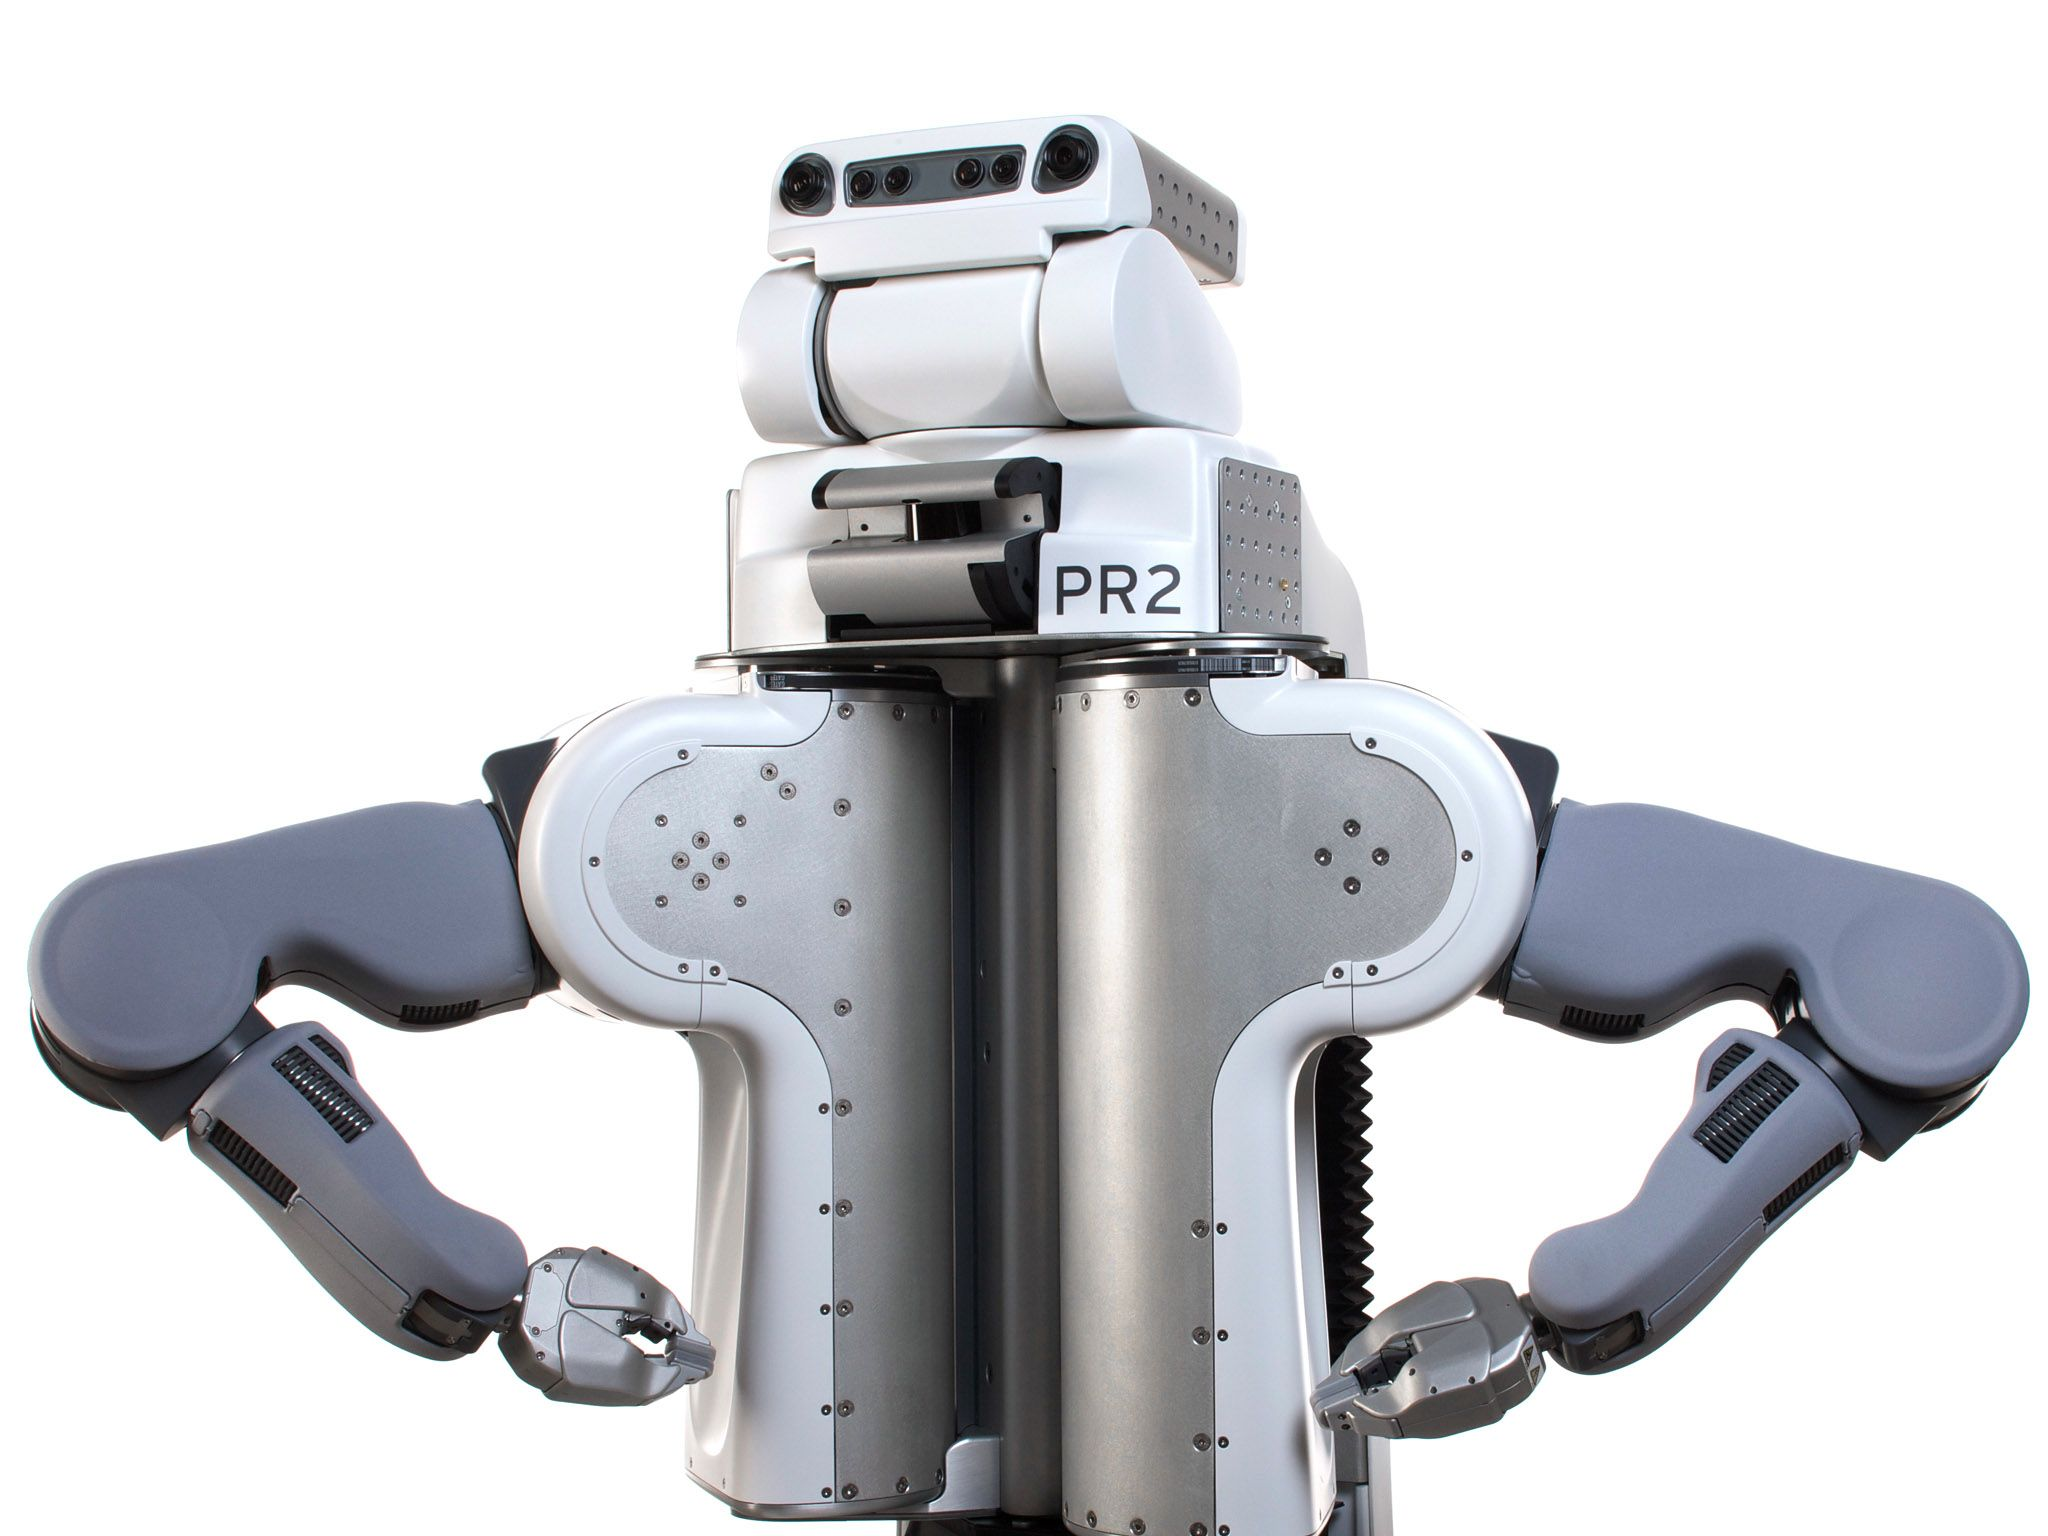
\includegraphics[scale=0.1]{Graphics/pr2.jpg}
	\caption{PR2 \cite{pr2}}
    \end{figure}

    \subsection{PyCram}
	\label{sec:pycram}
	\textit{PyCRAM} \cite{pycram} is a toolbox for designing, implementing and deploying software on autonomous robots. The framework provides various tools and libraries for aiding in robot software development as well as geometric reasoning and fast simulation mechanisms to develop cognition-enabled control programs that achieve high levels of robot autonomy.
    \textit{PyCRAM} \cite{pycram} is developed in the \textit{Python}-programming language with support for the \textit{ROS} \cite{ros} middleware which is used for communication with different software components as well as the robot.
    
    \textit{CRAM} \cite{beetz10cram} (Cognitive Robot Abstract Machine) is a software toolbox for the design, the implementation, and the deployment of cognition-enabled autonomous robots performing everyday manipulation activities.
	\textit{CRAM} \cite{beetz10cram} equips autonomous robots with lightweight reasoning mechanisms that can infer control decisions rather than requiring the decisions to be pre-programmed. 
	This way \textit{CRAM}-programmed autonomous robots are much more flexible, reliable, and general than control programs that lack such cognitive capabilities. 
	\textit{CRAM} \cite{beetz10cram} does not require the whole domain to be stated explicitly in an abstract knowledge base. Rather, it grounds symbolic expressions in the knowledge representation into the perception and actuation routines and into the essential data structures of the control programs. 

    \begin{figure}[H]
    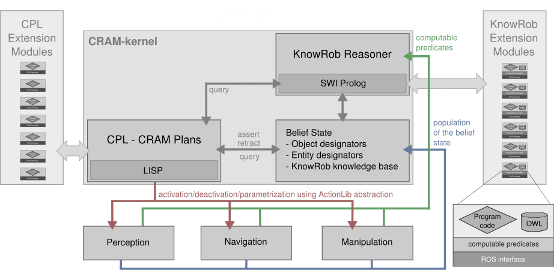
\includegraphics[scale=1.5]{Graphics/cram-language-architecture.png}
	\caption{\textit{CRAM} \cite{beetz10cram} Language Architecture}
    \end{figure}

	\subsection{PyBullet}
	\label{sec:pybullet}
	\textit{PyBullet}\cite{coumans2021} is an open-source physics engine and 3D simulation library used for robotics, machine learning, and computer graphics research. 
	It offers accurate physics simulation, 3D rendering, robotics support, and seamless integration with machine learning frameworks. 
	With a \textit{Python}-API and cross-platform compatibility, it's a versatile tool for simulating complex environments and interactions.
    
	\section{Knowledge Section: Ontologies and Rules}
    The parameters inferred for various robot actions come from a knowledge base. In the following, the principle of an ontology, as well as the concept of rules, which play a crucial role in parameter inference, will be introduced.
    \subsection{Ontology}
	Ontologies \cite{ontotext} are structured frameworks that provide a formal representation of knowledge within a specific domain. They play a crucial role in knowledge representation, facilitating the organization and sharing of information in a way that is both machine-readable and understandable by humans. 

    \begin{figure}[H]
        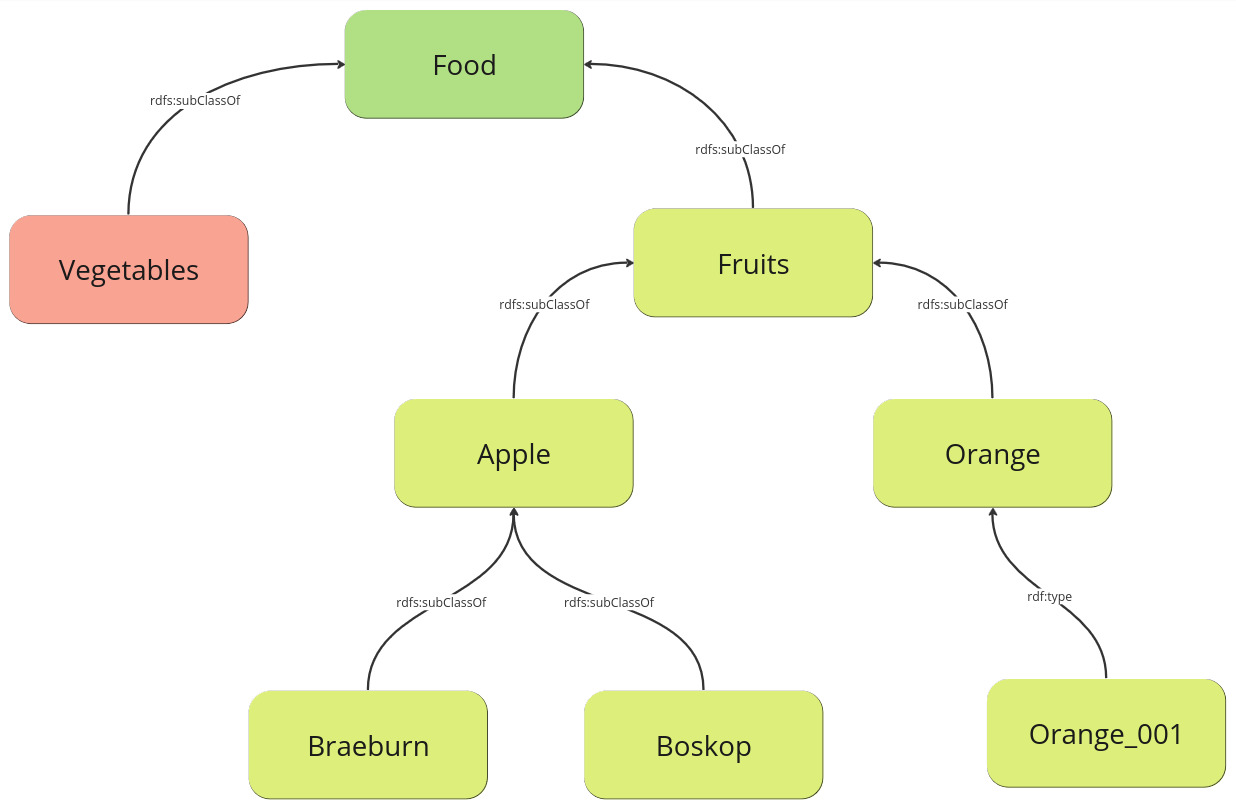
\includegraphics[scale=0.27]{Graphics/ontology.jpg}
		\caption{Ontology example}
    \end{figure}
	Key components of ontologies include:

	\begin{itemize}
		\item \textbf{Concepts/Classes}: These represent abstract or concrete entities within a domain. For example, in a food product ontology, \textit{Apple} and \textit{Orange} might be classes.
		\item \textbf{Properties/Roles}: These define the relationships between concepts. For instance, in a our example ontology, \textit{subClassOf} could be a property connecting individuals like \textit{Fruits} and \textit{Apple}.
		\item \textbf{Instances/Individuals}: These are specific members or examples of a class, \textit{Orange\_001} can be an instance of the class \textit{Orange}.
		\item \textbf{Axioms}: These are statements that describe the properties and relationships of the entities within the ontology. Axioms help define the logic and rules governing the domain.
		\item \textbf{Hierarchy}: Ontologies often organize concepts into a hierarchy, with more general concepts at the top and more specific ones below. This hierarchical structure aids in categorization and understanding.
		\item \textbf{Inference Rules}: These rules define how new information can be derived from existing information in the ontology. Inferences help systems reason and make deductions based on the knowledge encoded in the ontology.
	\end{itemize}
	We utilize ontologies in knowledge representation and reasoning systems to empower the robot with the ability to comprehend and handle information in a structured fashion for our specific objectives.

	\subsection{SWRL}
	\label{sec:SWRL}
	\textit{SWRL} \cite{Horrocks2004}, which stands for Semantic Web Rule Language, is a rule language that allows users to define rules about the relationships between classes and individuals in ontologies represented in the Web Ontology Language (\textit{OWL}). \textit{SWRL} \cite{Horrocks2004} is designed to be used in conjunction with \textit{OWL} to express complex relationships and infer new information based on existing knowledge.

	\textit{SWRL} \cite{Horrocks2004} Rules have a specific syntax and consist of two main components:
	\begin{itemize}
		\item \textbf{Antecedent (Body)}: This part of the rule specifies the conditions or constraints that must be satisfied for the rule to be applicable. It describes the current state of the ontology that triggers the rule.
		\item \textbf{Consequent (Head)}: This part defines the actions or inferences that should be taken if the conditions specified in the antecedent are satisfied. It describes the changes or additional information that should be inferred when the rule is triggered.
	\end{itemize}
	\textit{SWRL} \cite{Horrocks2004} supports various built-in predicates and functions, and users can create their own custom rules to suit their specific ontology. Some common elements in \textit{SWRL} \cite{Horrocks2004} rules include:
	\begin{itemize}
		\item \textbf{Individuals}: Refers to specific instances of classes in the ontology.
		\item \textbf{Class and Property Relationships}: Describes relationships between classes and properties in the ontology.
		\item \textbf{Built-in Predicates and Functions:} Includes operations such as arithmetic, string manipulation, and comparison functions that can be used in the rule conditions.
	\end{itemize}

	HIER NASER
	Here's a simple example of a \textit{SWRL} \cite{Horrocks2004} rule:
	\newline
	$Person(?x) ^ hasChild(?x, ?y) -> Grandparent(?x, ?z) ^ hasChild(?y, ?z)$
	\newline
	In this example:

	If an individual (?x) is a Person and has a child (?y),
	
	Then, infer that the individual (?x) is a Grandparent of another individual (?z), and the child (?y) is the parent of (?z).
	
	\textit{SWRL} \cite{Horrocks2004} rules are useful for expressing complex relationships and constraints within ontologies, enabling automated reasoning systems to make inferences and derive new knowledge from existing data.

	\section{Software Libraries}
\label{sec:Libraries}
\subsection{RDFLib}
\label{sec:RDFLib}
\textit{RDFLib} \cite{Krech_RDFLib_2023} is a \textit{Python}-package designed to work with \textit{Resource Description Framework (RDF)} data. \textit{RDF} is a standard model for data interchange on the web and is used to represent information in the form of subject-predicate-object triples. Key features of the library are:

\begin{itemize}
    \item \textbf{Parsing RDF Data}: \textit{RDFLib} can parse \textit{RDF}-data in various formats such as \textit{RDF/XML, N-Triples, Turtle}, and more.
    
    \item \textbf{Creating and Modifying RDF Graphs}: It allows you to create and manipulate \textit{RDF}-graphs, which consist of a collection of \textit{RDF}-triples. You can add, remove, or modify triples in the graph.
    
    \item \textbf{Querying RDF Data}: \textit{RDFLib} provides a \textit{SPARQL} query engine, allowing you to perform queries on \textit{RDF}-graphs using the \textit{SPARQL} query language.
    
    \item \textbf{Serializing RDF Data}: You can serialize \textit{RDF}-graphs back into different \textit{RDF}-formats using \textit{RDFLib}, making it easy to store or share \textit{RDF}-data.
    
    \item \textbf{Working with Ontologies}: It supports working with \textit{RDF}-vocabularies and ontologies, enabling the use of predefined classes and properties from existing ontologies like \textit{RDF}-schema (\textit{RDFS}) or the Web Ontology Language (\textit{OWL}).
    
    \item \textbf{Integration with Semantic Web Tools}: \textit{RDFLib} can be integrated with other semantic web tools and frameworks, allowing to build applications that leverage semantic web technologies.
\end{itemize}

\subsection{Flask}
\label{sec:flask}
\textit{Flask} \cite{grinberg2018flask} is a lightweight and flexible web framework for \textit{Python}, designed to make it easy to create web applications. It follows the \textit{WSGI} standard and the minimalist approach, offering essential tools and features for building web services and APIs. 

	\subsection{Owlready}
	\label{sec:OWLReady}
	One important library used for our implementation is \textit{Owlready} \cite{LAMY201711}. \textit{Owlready} \cite{LAMY201711} is a \textit{Python}-library designed for ontology-oriented programming. It facilitates the development, manipulation, and querying of ontologies using the Web Ontology Language (\textit{OWL}), a standard for representing knowledge in a machine-readable format. \textit{Owlready} \cite{LAMY201711} simplifies ontology-related tasks by providing a convenient and object-oriented interface for working with \textit{OWL} ontologies in \textit{Python}.

	Key features of the \textit{Owlready} \cite{LAMY201711} library include:

	\begin{itemize}
		\item \textbf{Object-Oriented Programming (OOP)}: \textit{Owlready} \cite{LAMY201711} adopts an object-oriented approach, allowing users to interact with ontology entities as \textit{Python}-objects. This makes it more intuitive for developers familiar with \textit{Pythons}-principles.
		\item \textbf{Ontology Loading and Parsing}: The library supports the loading and parsing of \textit{OWL} ontologies, making it easy to access and manipulate ontology data within \textit{Python}-scripts or applications.
		\item \textbf{Class and Individual Manipulation}: \textit{Owlready} \cite{LAMY201711} provides functionality for creating, modifying, and querying classes and individuals within an ontology. This allows for dynamic and programmatic management of ontology content.
		\item \textbf{Reasoning Support}: Depending on the version and features, \textit{Owlready} \cite{LAMY201711} may offer support for reasoning tasks. Reasoning involves deducing implicit information based on the logical relationships defined in the ontology.
		\item \textbf{Integration with \textit{RDFLib}}: \textit{Owlready} \cite{LAMY201711} may integrate with \textit{RDFLib}, another \textit{Python}-library commonly used for working with Resource Description Framework (\textit{RDF}-data). This integration enhances the capabilities of handling semantic data.
	\end{itemize}

	\subsection{WikiHow-Instruction-Extraction}
	\label{sec:WikiHow}
	
	\begin{wrapfigure}{r}{0.5\textwidth}
        \centering
        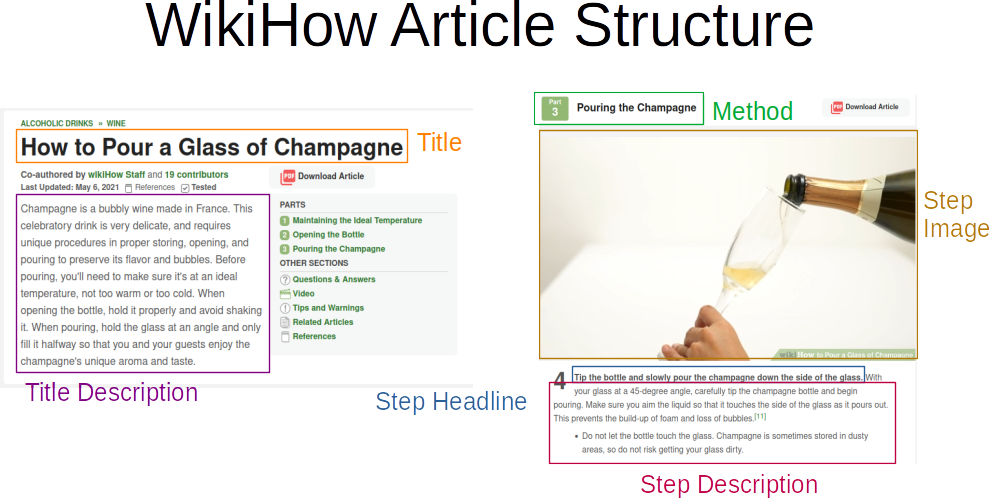
\includegraphics[width=0.48\textwidth]{Graphics/WikiHow Article Structure.png}
    \end{wrapfigure}
	\textit{WikiHow-Instruction-Extraction} \cite{wikihow-extraction}  is an extraction tool, that can collect informations from the WikiHow \cite{wikihow} corpus. 
	The goal of this tool is to analyse a WikiHow corpus using \textit{NLP} techniques to gather information about everyday tasks like \textit{Pouring}, \textit{Cutting} or \textit{Discarding}. 
	These information should support cognitive robots in understanding and parameterizing these tasks to better handle unknown tasks, working in underspecified environments and handling common task-object combinations.
	Every verb has its own class, in which the verb and the additionally desired hyponyms/synonyms are defined. These verbs serve as keywords for the search in the WikiHow \cite{wikihow} articles. Additionally, various parameters can be set, such as excluding different categories that are not relevant for the search.